\documentclass[]{article}
\usepackage{lmodern}
\usepackage{amssymb,amsmath}
\usepackage{ifxetex,ifluatex}
\usepackage{fixltx2e} % provides \textsubscript
\ifnum 0\ifxetex 1\fi\ifluatex 1\fi=0 % if pdftex
  \usepackage[T1]{fontenc}
  \usepackage[utf8]{inputenc}
\else % if luatex or xelatex
  \ifxetex
    \usepackage{mathspec}
  \else
    \usepackage{fontspec}
  \fi
  \defaultfontfeatures{Ligatures=TeX,Scale=MatchLowercase}
\fi
% use upquote if available, for straight quotes in verbatim environments
\IfFileExists{upquote.sty}{\usepackage{upquote}}{}
% use microtype if available
\IfFileExists{microtype.sty}{%
\usepackage{microtype}
\UseMicrotypeSet[protrusion]{basicmath} % disable protrusion for tt fonts
}{}
\usepackage[margin=1in]{geometry}
\usepackage{hyperref}
\hypersetup{unicode=true,
            pdftitle={How to use Join and Calculate Fields Tool},
            pdfauthor={Air Force Civic Engineering Center (AFCEC)},
            pdfborder={0 0 0},
            breaklinks=true}
\urlstyle{same}  % don't use monospace font for urls
\usepackage{color}
\usepackage{fancyvrb}
\newcommand{\VerbBar}{|}
\newcommand{\VERB}{\Verb[commandchars=\\\{\}]}
\DefineVerbatimEnvironment{Highlighting}{Verbatim}{commandchars=\\\{\}}
% Add ',fontsize=\small' for more characters per line
\usepackage{framed}
\definecolor{shadecolor}{RGB}{248,248,248}
\newenvironment{Shaded}{\begin{snugshade}}{\end{snugshade}}
\newcommand{\KeywordTok}[1]{\textcolor[rgb]{0.13,0.29,0.53}{\textbf{#1}}}
\newcommand{\DataTypeTok}[1]{\textcolor[rgb]{0.13,0.29,0.53}{#1}}
\newcommand{\DecValTok}[1]{\textcolor[rgb]{0.00,0.00,0.81}{#1}}
\newcommand{\BaseNTok}[1]{\textcolor[rgb]{0.00,0.00,0.81}{#1}}
\newcommand{\FloatTok}[1]{\textcolor[rgb]{0.00,0.00,0.81}{#1}}
\newcommand{\ConstantTok}[1]{\textcolor[rgb]{0.00,0.00,0.00}{#1}}
\newcommand{\CharTok}[1]{\textcolor[rgb]{0.31,0.60,0.02}{#1}}
\newcommand{\SpecialCharTok}[1]{\textcolor[rgb]{0.00,0.00,0.00}{#1}}
\newcommand{\StringTok}[1]{\textcolor[rgb]{0.31,0.60,0.02}{#1}}
\newcommand{\VerbatimStringTok}[1]{\textcolor[rgb]{0.31,0.60,0.02}{#1}}
\newcommand{\SpecialStringTok}[1]{\textcolor[rgb]{0.31,0.60,0.02}{#1}}
\newcommand{\ImportTok}[1]{#1}
\newcommand{\CommentTok}[1]{\textcolor[rgb]{0.56,0.35,0.01}{\textit{#1}}}
\newcommand{\DocumentationTok}[1]{\textcolor[rgb]{0.56,0.35,0.01}{\textbf{\textit{#1}}}}
\newcommand{\AnnotationTok}[1]{\textcolor[rgb]{0.56,0.35,0.01}{\textbf{\textit{#1}}}}
\newcommand{\CommentVarTok}[1]{\textcolor[rgb]{0.56,0.35,0.01}{\textbf{\textit{#1}}}}
\newcommand{\OtherTok}[1]{\textcolor[rgb]{0.56,0.35,0.01}{#1}}
\newcommand{\FunctionTok}[1]{\textcolor[rgb]{0.00,0.00,0.00}{#1}}
\newcommand{\VariableTok}[1]{\textcolor[rgb]{0.00,0.00,0.00}{#1}}
\newcommand{\ControlFlowTok}[1]{\textcolor[rgb]{0.13,0.29,0.53}{\textbf{#1}}}
\newcommand{\OperatorTok}[1]{\textcolor[rgb]{0.81,0.36,0.00}{\textbf{#1}}}
\newcommand{\BuiltInTok}[1]{#1}
\newcommand{\ExtensionTok}[1]{#1}
\newcommand{\PreprocessorTok}[1]{\textcolor[rgb]{0.56,0.35,0.01}{\textit{#1}}}
\newcommand{\AttributeTok}[1]{\textcolor[rgb]{0.77,0.63,0.00}{#1}}
\newcommand{\RegionMarkerTok}[1]{#1}
\newcommand{\InformationTok}[1]{\textcolor[rgb]{0.56,0.35,0.01}{\textbf{\textit{#1}}}}
\newcommand{\WarningTok}[1]{\textcolor[rgb]{0.56,0.35,0.01}{\textbf{\textit{#1}}}}
\newcommand{\AlertTok}[1]{\textcolor[rgb]{0.94,0.16,0.16}{#1}}
\newcommand{\ErrorTok}[1]{\textcolor[rgb]{0.64,0.00,0.00}{\textbf{#1}}}
\newcommand{\NormalTok}[1]{#1}
\usepackage{graphicx,grffile}
\makeatletter
\def\maxwidth{\ifdim\Gin@nat@width>\linewidth\linewidth\else\Gin@nat@width\fi}
\def\maxheight{\ifdim\Gin@nat@height>\textheight\textheight\else\Gin@nat@height\fi}
\makeatother
% Scale images if necessary, so that they will not overflow the page
% margins by default, and it is still possible to overwrite the defaults
% using explicit options in \includegraphics[width, height, ...]{}
\setkeys{Gin}{width=\maxwidth,height=\maxheight,keepaspectratio}
\IfFileExists{parskip.sty}{%
\usepackage{parskip}
}{% else
\setlength{\parindent}{0pt}
\setlength{\parskip}{6pt plus 2pt minus 1pt}
}
\setlength{\emergencystretch}{3em}  % prevent overfull lines
\providecommand{\tightlist}{%
  \setlength{\itemsep}{0pt}\setlength{\parskip}{0pt}}
\setcounter{secnumdepth}{0}
% Redefines (sub)paragraphs to behave more like sections
\ifx\paragraph\undefined\else
\let\oldparagraph\paragraph
\renewcommand{\paragraph}[1]{\oldparagraph{#1}\mbox{}}
\fi
\ifx\subparagraph\undefined\else
\let\oldsubparagraph\subparagraph
\renewcommand{\subparagraph}[1]{\oldsubparagraph{#1}\mbox{}}
\fi

%%% Use protect on footnotes to avoid problems with footnotes in titles
\let\rmarkdownfootnote\footnote%
\def\footnote{\protect\rmarkdownfootnote}

%%% Change title format to be more compact
\usepackage{titling}

% Create subtitle command for use in maketitle
\newcommand{\subtitle}[1]{
  \posttitle{
    \begin{center}\large#1\end{center}
    }
}

\setlength{\droptitle}{-2em}
  \title{How to use Join and Calculate Fields Tool}
  \pretitle{\vspace{\droptitle}\centering\huge}
  \posttitle{\par}
  \author{Air Force Civic Engineering Center (AFCEC)}
  \preauthor{\centering\large\emph}
  \postauthor{\par}
  \predate{\centering\large\emph}
  \postdate{\par}
  \date{19 April, 2018}


\begin{document}
\maketitle

\section{Overview}\label{overview}

The ArcGIS Python Script Tool ``Join Fields and Calculate'' may be used
to update the destination values in a target feature layer field with
the values in another table's fields using a common key (join). This
script will perform similarly as if you joined a table to a feature
class to calculate a certain field based on another field in the joined
table.

\section{Parameters}\label{parameters}

The tool has 8 parameters: 1. Transfer\_From (data type: Table View) -
Which table are do you want to transfer data from? This parameter must
be the path to a table(e.g.: Comma-separated Values (.csv) file, Excel
Workbook (.xlsx) Sheet, Esri geodatabase table, etc.). This table will
act as `source' data.

\begin{enumerate}
\def\labelenumi{\arabic{enumi}.}
\setcounter{enumi}{1}
\item
  Using\_Join\_Field (data type: Field) - From the source table, which
  field should be used to joinwith another feature class' attributes?
  This will provide the `key' to transfer data from the source table to
  the target table.
\item
  Source\_Field (data type: Field) -From the source table, which field's
  data do you want to transfer to the target table? This field's data
  will be updated in the target feature class that have matching fields.
\item
  Destination\_Feature (data type: Feature Layer or Feature Class) -
  Which feature class do you want to transfer data to? This parameter
  must be the path to a Esri Feature Class or Feature Layer. This table
  will act as `target' data source.
\item
  Destination\_Join\_Field (data type: Field) - From the target table,
  which field should be used to joinwith another feature class'
  attributes? This will provide the `key' to transfer data from the
  source table to the target table.
\item
  Destination\_Field (data type: Field) - From the target table, which
  field's data do you want to transfer from the source table? This
  field's data will be updated from the source table that have matching
  fields using the join fields provided.
\item
  Where\_Clause (data type: String) - How should the source values be
  filtered? Default is ``IS NOT NULL'', otherwise you will overwrite the
  target features will null values.
\item
  Remove\_Leading\_Zeros (data type: Boolean) - Do you want to remove
  leading zeros from the Source Join Field prior to `joining' the
  tables?
\end{enumerate}

\section{How to Use}\label{how-to-use}

\begin{enumerate}
\def\labelenumi{\arabic{enumi}.}
\tightlist
\item
  Begin by opening the toolbox
\end{enumerate}

\begin{Shaded}
\begin{Highlighting}[]
\CommentTok{# All defaults}
\KeywordTok{include_graphics}\NormalTok{(}\StringTok{"C:}\CharTok{\textbackslash{}\textbackslash{}}\StringTok{Users}\CharTok{\textbackslash{}\textbackslash{}}\StringTok{stevenconnorg}\CharTok{\textbackslash{}\textbackslash{}}\StringTok{Documents}\CharTok{\textbackslash{}\textbackslash{}}\StringTok{knight-federal-solutions}\CharTok{\textbackslash{}\textbackslash{}}\StringTok{CIP_DataReview}\CharTok{\textbackslash{}\textbackslash{}}\StringTok{tutorial-images}\CharTok{\textbackslash{}\textbackslash{}}\StringTok{joinCalc-open_tool.jpg"}\NormalTok{)}
\end{Highlighting}
\end{Shaded}

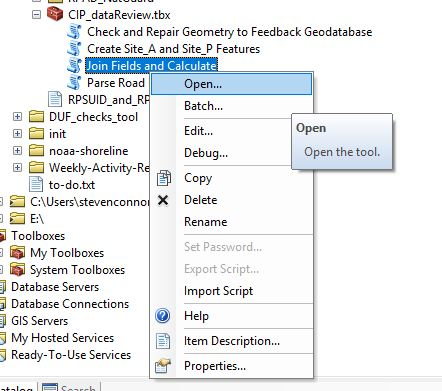
\includegraphics[width=6.14in]{C:\Users\stevenconnorg\Documents\knight-federal-solutions\CIP_DataReview\tutorial-images\joinCalc-open_tool}

\begin{enumerate}
\def\labelenumi{\arabic{enumi}.}
\setcounter{enumi}{1}
\tightlist
\item
  Fill out the parameters
\end{enumerate}

\begin{Shaded}
\begin{Highlighting}[]
\CommentTok{# All defaults}
\KeywordTok{include_graphics}\NormalTok{(}\StringTok{"C:}\CharTok{\textbackslash{}\textbackslash{}}\StringTok{Users}\CharTok{\textbackslash{}\textbackslash{}}\StringTok{stevenconnorg}\CharTok{\textbackslash{}\textbackslash{}}\StringTok{Documents}\CharTok{\textbackslash{}\textbackslash{}}\StringTok{knight-federal-solutions}\CharTok{\textbackslash{}\textbackslash{}}\StringTok{CIP_DataReview}\CharTok{\textbackslash{}\textbackslash{}}\StringTok{tutorial-images}\CharTok{\textbackslash{}\textbackslash{}}\StringTok{joinCalc-tool_params.jpg"}\NormalTok{)}
\end{Highlighting}
\end{Shaded}

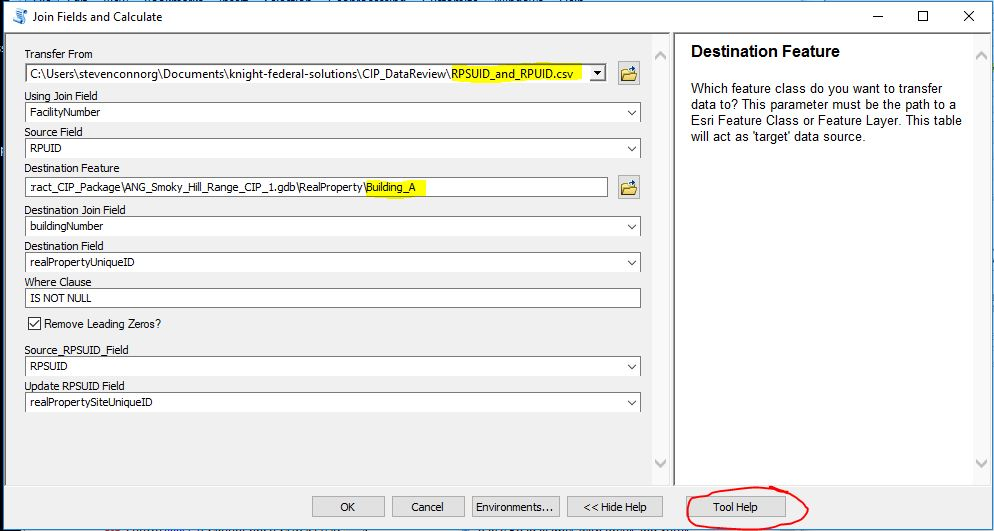
\includegraphics[width=14.46in]{C:\Users\stevenconnorg\Documents\knight-federal-solutions\CIP_DataReview\tutorial-images\joinCalc-tool_params}

\begin{enumerate}
\def\labelenumi{\arabic{enumi}.}
\setcounter{enumi}{2}
\tightlist
\item
  View the update results
\end{enumerate}

\begin{Shaded}
\begin{Highlighting}[]
\CommentTok{# All defaults}
\KeywordTok{include_graphics}\NormalTok{(}\StringTok{"C:}\CharTok{\textbackslash{}\textbackslash{}}\StringTok{Users}\CharTok{\textbackslash{}\textbackslash{}}\StringTok{stevenconnorg}\CharTok{\textbackslash{}\textbackslash{}}\StringTok{Documents}\CharTok{\textbackslash{}\textbackslash{}}\StringTok{knight-federal-solutions}\CharTok{\textbackslash{}\textbackslash{}}\StringTok{CIP_DataReview}\CharTok{\textbackslash{}\textbackslash{}}\StringTok{tutorial-images}\CharTok{\textbackslash{}\textbackslash{}}\StringTok{joinCalc-results.jpg"}\NormalTok{)}
\end{Highlighting}
\end{Shaded}

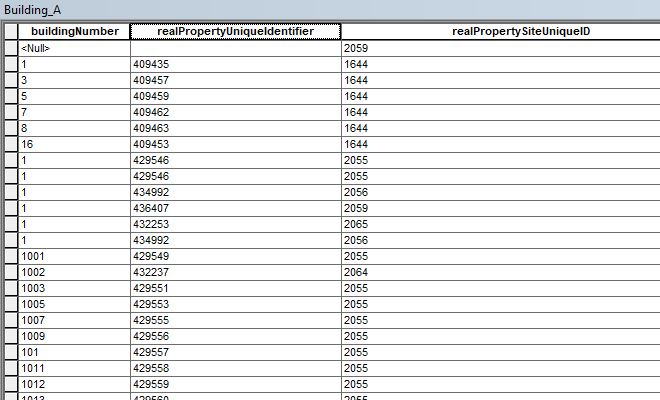
\includegraphics[width=5.96in]{C:\Users\stevenconnorg\Documents\knight-federal-solutions\CIP_DataReview\tutorial-images\joinCalc-results}

\pagebreak

\section{Production Info}\label{production-info}

For posterity, development information used to compile this report is
listed below.

\begin{verbatim}
## R version 3.4.1 (2017-06-30)
## Platform: x86_64-w64-mingw32/x64 (64-bit)
## Running under: Windows >= 8 x64 (build 9200)
## 
## Matrix products: default
## 
## locale:
## [1] LC_COLLATE=English_United States.1252 
## [2] LC_CTYPE=English_United States.1252   
## [3] LC_MONETARY=English_United States.1252
## [4] LC_NUMERIC=C                          
## [5] LC_TIME=English_United States.1252    
## 
## attached base packages:
## [1] stats     graphics  grDevices utils     datasets  methods   base     
## 
## other attached packages:
##  [1] bookdown_0.7    rmarkdown_1.9   knitr_1.20      tinytex_0.5    
##  [5] devtools_1.13.4 backports_1.1.2 digest_0.6.15   anchors_3.0-8  
##  [9] MASS_7.3-49     rgenoud_5.8-1.0 bibtex_0.4.2    purrr_0.2.4    
## [13] Rcpp_0.12.16    ggmap_2.6.1     sf_0.6-1        markdown_0.8   
## [17] stringr_1.3.0   DT_0.4          leaflet_1.1.0   dplyr_0.7.4    
## [21] ggplot2_2.2.1   rprojroot_1.3-2 packrat_0.4.9-1
## 
## loaded via a namespace (and not attached):
##  [1] xfun_0.1          reshape2_1.4.3    lattice_0.20-35  
##  [4] colorspace_1.3-2  htmltools_0.3.6   yaml_2.1.18      
##  [7] rlang_0.2.0       e1071_1.6-8       pillar_1.2.1     
## [10] withr_2.1.2       glue_1.2.0        DBI_0.8          
## [13] sp_1.2-7          bindrcpp_0.2.2    jpeg_0.1-8       
## [16] bindr_0.1.1       plyr_1.8.4        munsell_0.4.3    
## [19] gtable_0.2.0      htmlwidgets_1.0   RgoogleMaps_1.4.1
## [22] mapproj_1.2.6     evaluate_0.10.1   memoise_1.1.0    
## [25] httpuv_1.3.6.2    crosstalk_1.0.0   class_7.3-14     
## [28] proto_1.0.0       xtable_1.8-2      geosphere_1.5-7  
## [31] udunits2_0.13     scales_0.5.0      classInt_0.1-24  
## [34] mime_0.5          rjson_0.2.15      png_0.1-7        
## [37] stringi_1.1.7     shiny_1.0.5       grid_3.4.1       
## [40] tools_3.4.1       magrittr_1.5      maps_3.3.0       
## [43] lazyeval_0.2.1    tibble_1.4.2      pkgconfig_2.0.1  
## [46] assertthat_0.2.0  R6_2.2.2          units_0.5-1      
## [49] compiler_3.4.1
\end{verbatim}


\end{document}
